%\documentclass[options]{class}
\documentclass[12pt, twoside]{report}

%Paquete de Idioma
\usepackage[spanish]{babel}

%Codificación Alfabeto
\usepackage[utf8]{inputenc}

%Codificación de Fuente
\usepackage[T1]{fontenc}

%Índice
\usepackage{makeidx}

%Gráficos
\usepackage{graphicx}
\usepackage{float} 
%\usepackage{xcolor} 

%Matemática
\usepackage{amsmath}
\usepackage{amsfonts}
\usepackage{amssymb}
\usepackage{amstext} 

%Color en tablas! NUEVO.
\usepackage[table]{xcolor}
\usepackage{tabularx}
\usepackage{float}

%Código en C
\usepackage{listings}

%Anexos
\usepackage{appendix}
%Estilo de Página Numeración superior
%\pagestyle{headings}

%un estilo propio
\usepackage{fancyhdr}
\setlength{\headheight}{15pt}

\pagestyle{fancy}
\renewcommand{\chaptermark}[1]{ \markboth{\chaptername\ \thechapter: #1}{} }
\renewcommand{\sectionmark}[1]{ \markright{ Sección \thesection. #1}{} }

\fancyhf{}
\fancyhead[LE,RO]{\thepage}
\fancyhead[RE]{\textit{ \nouppercase{\leftmark}} }
\fancyhead[LO]{\textit{ \nouppercase{\rightmark}} }
\fancyfoot[CE]{\textit{\textcopyright 2014 Laboratorio de Sistemas Embebidos\\
	                    UPAEP} }
\fancyfoot[CO]{\textit{LSE001-2014 \\
		Elaboró: Dr. Casimiro Gómez González} }	            
\fancypagestyle{plain}{ %
	\fancyhf{} % remove everything
	\renewcommand{\headrulewidth}{0pt} % remove lines as well
	\renewcommand{\footrulewidth}{0pt}
}

%Hiperlinks \href{url}{text}
\usepackage[pdftex]{hyperref}

\usepackage{cite} % para contraer referencias

%Titulo
\title{LSE001-2014: Sistemas Operativos en Tiempo Real}
\author{Dr. Casimiro Gómez González$^{1}$,Oscar Navarrete Aguilar$^{2}$\\
	Facultad de Electrónica, UPAEP\\
               Correos: $^{1}$casimiro.gomez@upaep.mx,$^{2}$oscar.navarrete@upaep.edu.mx\\
               Tel: 222 229 9428}
	
\date{Otoño 2014}

\begin{document}

\maketitle

\chapter*{Prólogo}

En el presente reporte se realiza un estudio de los sistemas operativos en tiempo real con el objetivo de aplicarlos en las tarjetas embebidas con microcontroladores ARM. Se ha elegido la plataforma \textit{CMSIS-RTOS RTX} de \textbf{Keil} y el microcontrolador \textit{LPC4357}. Se describe la aplicación de los sistemas operativos en tiempo real para un satélite \textbf{CubeSat}. Este documento se inicio en el otoño 2014 y estará en actualización continua.


\begin{flushright}
	
	El autor\\
	Casimiro Gómez González\\
	Doctor en Ingeniería Mecatrónica
\end{flushright}

\tableofcontents


\chapter{Introducción}

Los microprocesadores arribaron en 1970. Los sistemas operativos encontraron aplicación rápida en las sistemas basados en microprocesador. Para mediados de 1980 pocas de estas implementaciones usadas se pueden describir como sistemas operativos en tiempo real diseñados formalmente.Dos factores afectan la aceptación de los sistemas operativos en tiempo real, uno debido a los limites de la máquina, y los otros a la cultura de diseño alrededor de los microcontroladores. Los primeros microprocesador estaban bastante limitados en sus habilidades computacionales, velocidad de operación y capacidades de memoria. Tratar de establecer la estructura de un sistema operativo bajo estas bases es muy difícil. Sin embargo, la mayoría de estos sistemas operativos embebidos programados tienen poco o ningún relación con sistemas operativos \cite{Cooling2014}.

\section{Produciendo software de calidad}
Si se desea diseñar software de alta calidad, este debe tener las siguientes características:

\begin{itemize}
	\item Debe realizar su trabajo correctamente (\textbf{funcionalmente correcto})
	\item Debe realizar su trabajo en el tiempo correcto (\textbf{temporalmente correcto})
	\item Su comportamiento debe ser predecible
	\item Su comportamiento debe ser consistente
	\item El código no debe ser difícil de mantener (baja complejidad)
	\item Lo correcto del código puede ser analizado (análisis estático)
	\item El comportamiento del código puede ser analizado (análisis de cobertura) 
	\item El comportamiento en tiempo de ejecución debe ser predecible
	\item Los requerimientos de memoria debe ser predecibles
	\item El código puede, si es necesario, ser validado de acuerdo con estándares relevantes. 
	
\end{itemize} 

\section{Modelando Software}
Existen diferentes etapas para producir un programa ejecutable, como se indica en la figura \ref{cap1:001}.

%\begin{figure}
%\centering
%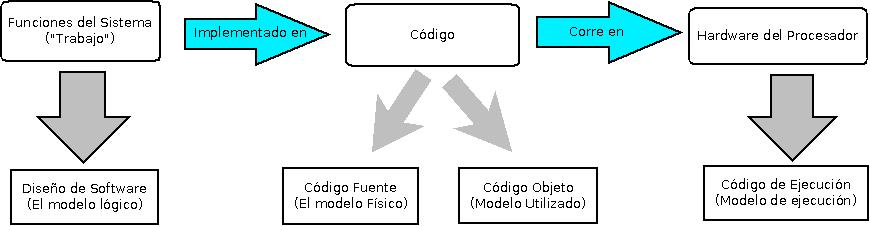
\includegraphics[width=100mm]{runtime}
%\caption{Etapas desde el diseño hasta la ejecución}
%\label{cap1:001}
%\end{figure}

Primero el diseño del software, resulta en el diseño o modelo lógico. Esto es implementado como código fuente, el modelo físico. El código fuente es compilado, enlazado y construido a un código objeto, el modelo bajado (deployment model). Finalmente el código objeto es cargado en el procesador y despues ejecutado, el modelo de ejecución. 
El modelo del código nos proporciona un visión estática del software. En contraste con el modelo de ejecución, una combinación de código, datos y procesador, representa software en ejecución. Esto se define como un proceso de software, también conocida como una tarea en el mundo de los embebidos. En palabras simples, una tarea representa la ejecución de un programa secuencial simple. Por lo regular al modelo de ejecución también se le llama modelo de tareas.

%\begin{figure}
%\centering
%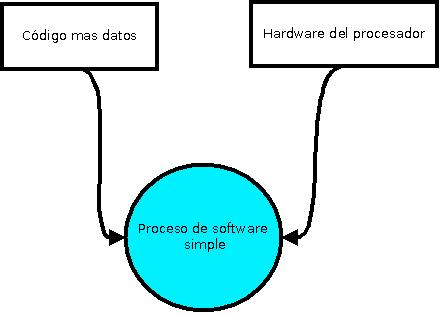
\includegraphics[width=80mm]{runtimemodel}
%\caption{El modelo de ejecución del proceso de software}
%\label{cap1:002}
%\end{figure}

\section{La importancia del tiempo y el temporizado}
En sistemas electrónicos analógicos todas las operaciones pueden, si se requiere, realizarse simultáneamente (concurrentemente), no solamente eso, sino que el procesamiento es hecho instantáneamente. Pero esto no es posible en sistemas basados en procesador ya que este es fundamentalmente discreto en sus operaciones:

\begin{itemize}
	\item Un procesador puede hacer solamente una cosa a tiempo (una maquina secuencial) y
	\item Las operaciones toman tiempo - las cosas no suceden instantáneamente
\end{itemize}

Estos son dos factores que causan muchas angustias en nuestro trabajo de diseño. Y esta es la razón por lo cual si esta diseñando sin conocer tus necesidades de tiempo, debes estar preparado para sorpresas desagradables.

Con esto en mente, los primeros diseños tenían las siguientes características:
\begin{itemize}
	\item Es ejecutado en un lazo continuo
	\item Termina su trabajo en cada lazo (Semantica de ejecutar hasta completar)
	\item Toma tiempo para completar su trabajo (Tiempo de ejecución de tareas- $Te$)
	\item Es repetido a intervalos regulares o periodos (operaciones periodicas - $Tp$)
	\item No hacer nada mientras esta retardado (tiempo desperdiciado $Ts$)
	\item Necesita un mecanismo de temporizado para controlar el periodo de tiempo 
\end{itemize}

En este diseño en particular $Tp$ y $Td$ son requisitos del sistema, $Te$ depende de nuestro código de solución y $Ts$ es nuestro tiempo limite, como puede verse en la figura . Por ejemplo, suponiendo que $Tp$ es $100ms$ y $Te$ es $5ms$, esto nos da un valor de $Ts$ de $95ms$. Esto quiere decir que el procesador esta ejecutando código por $5ms$ cada $100ms$, una utilización ($U$) de $5$\%. 

%\begin{figure}
%\centering
%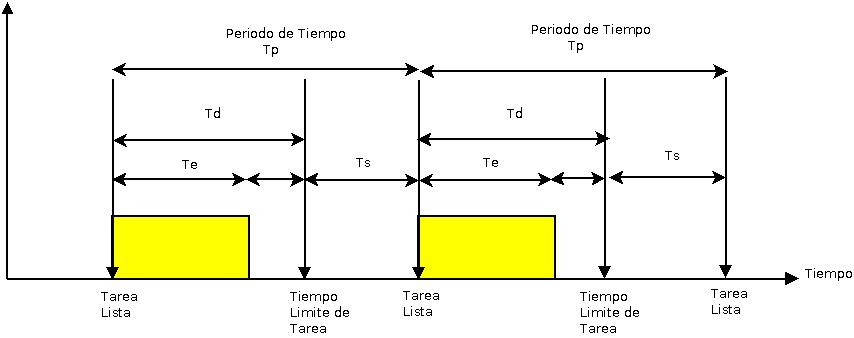
\includegraphics[width=100mm]{timing}
%\caption{Algunas definiciones básicas del Temporizado de Tareas}
%\label{cap1:003}
%\end{figure}
Primero, en los sistemas embebidos se pretende que las tareas se ejecuten hasta ser completadas cada vez que sean activadas. Segundo, en los sitemas prácticos debe haber un tiempo de espera $Ts$. Tercero, por el hecho de que un código se pueda ejecutar dentro de un periodo de tiempo esto no significa que su rendimiento sea aceptable. El retardo de tiempo del procesamiento de entrada-salida puede causar problemas en el comportamiento de todo el sistema.


\section{Manejando múltiples trabajos}
Para manejar trabajos concurrentes independientes, lo cual significa que tenemos diferentes trabajos que en el mundo real pueden:
\begin{enumerate}
	\item Ser atendidos a intervalos regulares - Funciones periódicas
	\item Ser atendidos en tiempos aleatorios - Funciones asíncronas o aperiodicas
	\item Ser procesados simultaneamente
	\item Muy diferentes necesidades de temporizado
\end{enumerate}

\section{Usando Interrupciones como máquina de ejecución}

Un \textbf{timer} se dispara, un interruptor se presiona, un dispositivo periférico necesita atención, son eventos típicos del mundo real en sistemas basados en computadoras. Hay, de hecho, solamente dos maneras de detectar estos eventos: Buscando estos eventos (polling) o enviando una señal directamente a el procesador (interrupciones de hardware).

A diferencia de los métodos anteriores cuando se usaba el polling dentro de una unidad secuencial de programa, ahora se buscan las interrupciones de hardware, una señal electrónica que es aplicada al procesador. Cuando la interrupción es generada se llama a una respuesta predeterminada (la cual es predefinida por el programador)  para ejecutar un software específico. Así que la interrupción puede ser vista como una máquina de ejecución de una pieza particular de software.

Así que lo que tenemos es una ejecución aparentemente concurrente de un conjunto individual de procesos (tareas), llamado ``cuasi-concurrencia''. En otras palabras, usando interrupciones, podemos correr múltiples tareas simultáneamente: una forma de multitareas simple. De esta forma se puede concluir que:

\begin{enumerate}
	\item Las interrupciones son mecanismos habilitados por llaves que permiten al diseño trabajar
	\item Las interrupciones simplifican el diseño funcional del sistema
	\item Las interrupciones simplifican el manejo de diferentes temporizados y requisitos de respuestas
	\item El comportamiento actual en tiempo de ejecución no puede ser predicho o analizado estáticamente
\end{enumerate}

\chapter{Empezando a crear proyectos con $ \mu $Vision de Keil}

En el presente capítulo se explica de forma detallada los pasos necesarios para compilar y cargar un proyecto usando el Software  \textit{$\mu $Vision}  y la plataforma \textit{CMSIS-RTOS RTX}, ambos de \textbf{Keil}, así como del microcontrolador \textit{LPC4357} 

\section{Instalando el software}

El software se encuentra disponible en la página \url{https://www.keil.com/download/product/} seleccionando el producto \textbf{MDK-ARM v5}. Al terminar la descarga y la instalación, se abre la interfaz. A continuación es necesario instalar los paquetes necesarios para el microcontrolador. Para ello se abre el complemento llamado \textbf{Pack Installer} y se busca el microcontrolador que se encuentra en \textbf{NXP -> LPC4300 Series -> LPC435x -> LPC4357}. Del lado izquierdo aparecerán los paquetes necesarios para instalar. Se da click en los botones correspondientes. En la figura \ref{cap1:001} se muestran estas opciones.

\begin{figure}[H]
	\centering
	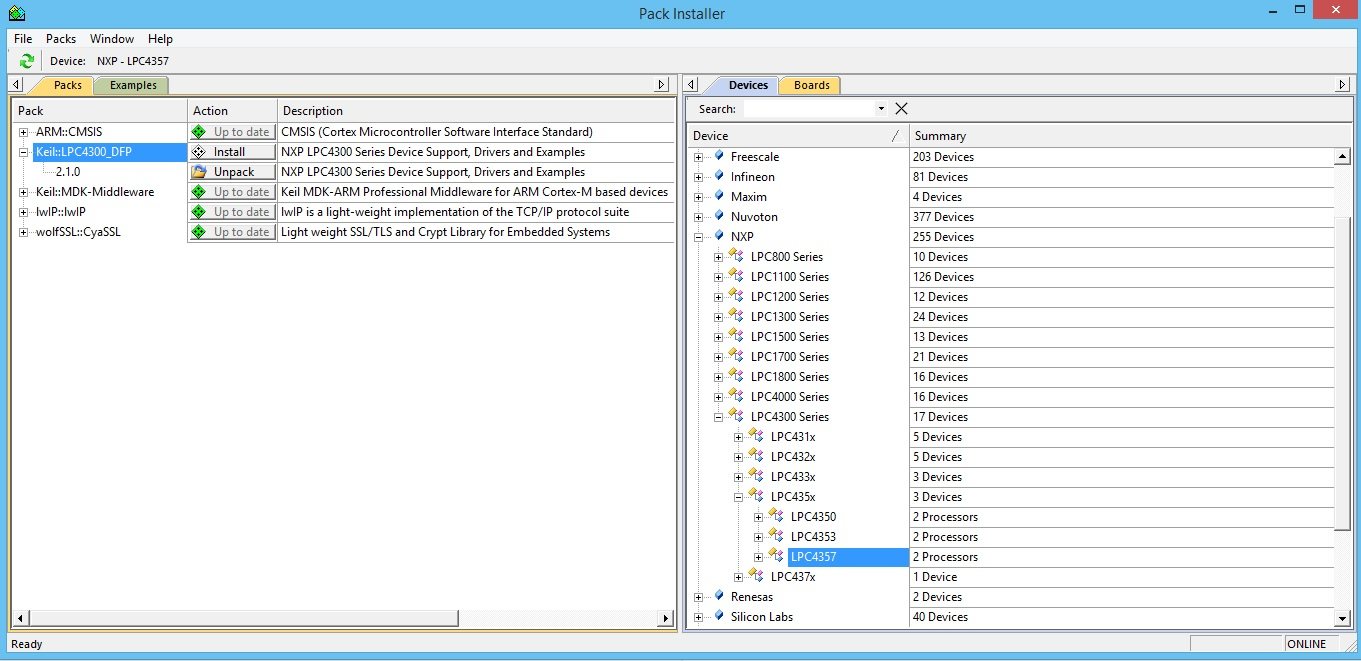
\includegraphics[width=100mm]{paqmicro}
	\caption{Instalación de paquetes del microcontrolador}
	\label{cap1:001}
\end{figure}

\section{Creación del proyecto}

Para crear un nuevo proyecto en \textit{$\mu$vision}, seguimos los siguientes pasos: \textbf{Barra de herramientas -> Project -> New $\mu$vision Project...}. En seguida se selecciona la carpeta en donde se quiere crear. Se recomienda tener una carpeta general y dentro de esta, exista una carpeta para cada proyecto debido al número de elementos creados por proyecto. Al seleccionar la carpeta y asingarle un nombre al proyecto, aparecerá una ventana como la de la figura \ref{cap1:002}. En seguida se selecciona el microcontrolador que se encuentra en \textbf{NXP -> LPC4300 Series -> LPC435x -> LPC4357 -> LPC4357: Cortex-M4} y se da click en \textbf{OK}.

\begin{figure}[H]
	\centering
	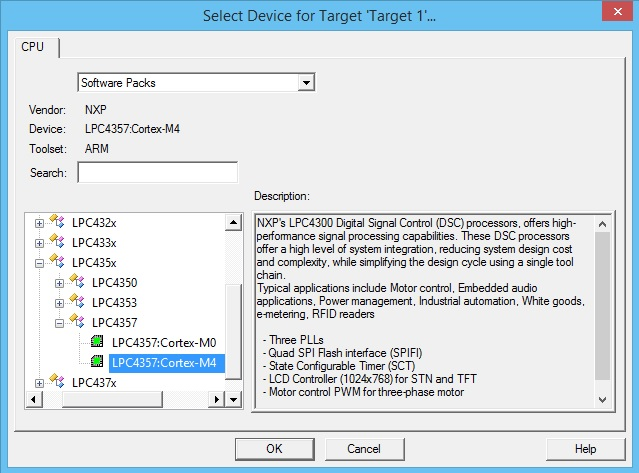
\includegraphics[width=100mm]{selecmicro}
	\caption{Selección del microcontrolador}
	\label{cap1:002}
\end{figure}

Para finalizar esta parte, es necesario seleccionar los Componentes del Software esenciales para el proyecto. En este caso, se encenderán los leds de la tarjeta MCB4300 usando la plataforma CMSIS-RTOS, para ello se necesitarán de los siguientes elementos: \textbf{Board Support -> LED(API) -> LED} , \textbf{CMSIS -> CORE} , \textbf{CMSIS -> RTOS(API) -> Keil RTX} , \textbf{Device -> GPIO} , \textbf{SCU} , \textbf{Startup} . En la figura \ref{cap1:003} se muestran los Componentes seleccionados. Al finalizar de seleccionar todos se da click en \textbf{OK}.

\begin{figure}[H]
	\centering
	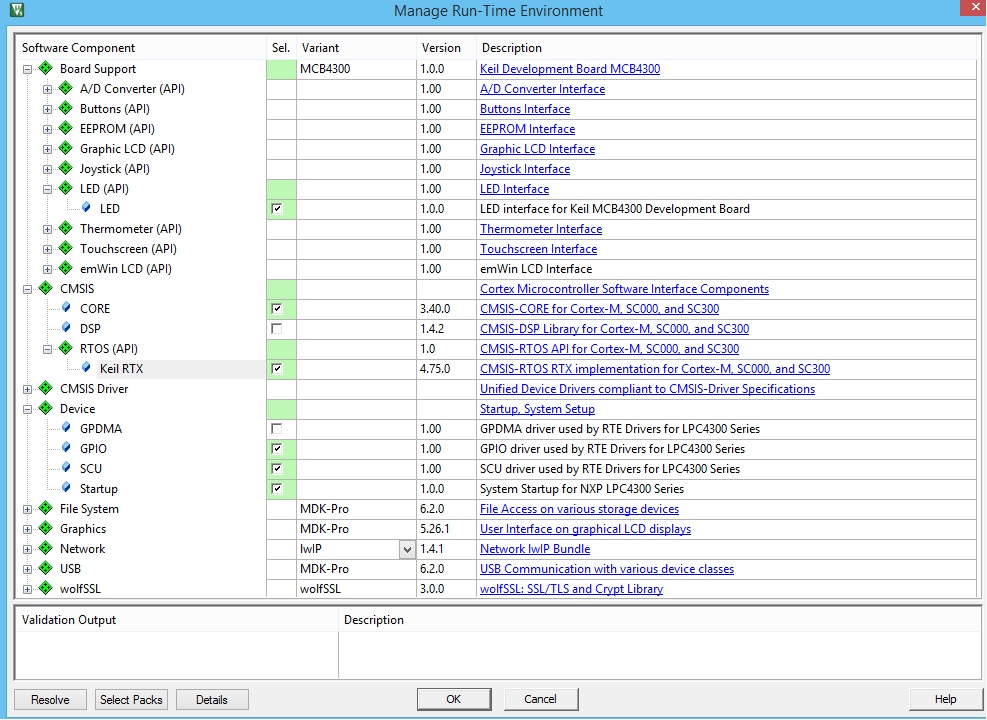
\includegraphics[width=100mm]{comrtos}
	\caption{Componentes necesarios para proyecto}
	\label{cap1:003}
\end{figure}

\section{Configuraciones básicas}

Se observa en la interfaz de $\mu$Vision que ya se encuentran los componentes necesarios para el proyecto. El siguiente paso es definir un nombre para la carpeta objetivo y para el grupo de fuente. Para ello se da click en la carpeta que por defecto se llama \textbf{Target 1} y a continuación en \textbf{Manage Project Items...} En la pestaña de \textbf{Project Items} se encuentran tres ventanas. En la primera ventana llamada \textbf{Project Targets} se da click en el botón \textbf{New (Insert)} y se escribe el nuevo nombre del proyecto. Al terminar, se selecciona el anterior nombre y se elimina con el botón \textbf{Delete (Delete)}. Se repite el mismo procedimiento para el nombre del grupo. Todas estas configuraciones se muestran en la figura \ref{cap1:004}. Al finalizar se da click en \textbf{OK}.

\begin{figure}[H]
	\centering
	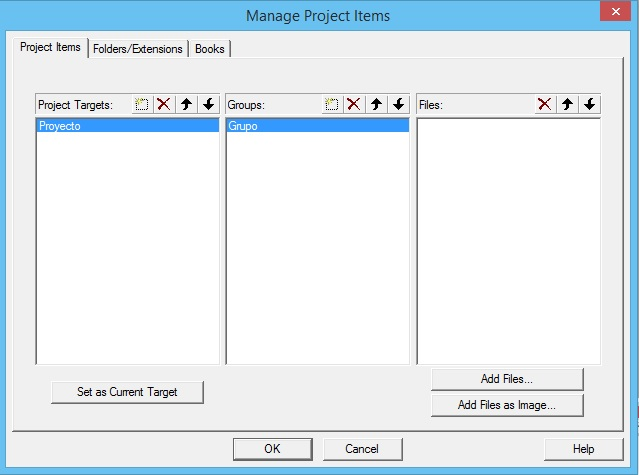
\includegraphics[width=100mm]{progrupo}
	\caption{Configuración de objetos del proyecto}
	\label{cap1:004}
\end{figure}

Se observa que ahora ya tienen otro nombre las carpetas del proyecto. Se prosigue a crear el archivo \textbf{main.c} para ello en la barra de herramientas se da click en \textbf{File} y en \textbf{New...}. En el \textbf{Anexo I} de este trabajo se encuentra un código de ejemplo que se puede ocupar para compilar y crear el primer proyecto, esto con el fin de enfocarse a la correcta realización del proyecto . Más adelante se explicarán a detalle las funciones y comandos necesarios de la plataforma CMSIS-RTOS.

Se guarda el código dando click en \textbf{File} y posteriormente en \textbf{Save As} en la misma carpeta del proyecto. El archivo se guarda con extensión \textbf{.c}. Ahora se da click derecho en la carpeta de grupo y se selecciona la opción \textbf{Add Existing Files to Group}. Se agrega el archivo que se acaba de guardar. Ahora ya aparecerá agregado en la lista debajo de la carpeta del grupo. 

Ahora es necesario realizar un par de modificaciones más a las configuraciones que trae el software por defecto. Para ello se da click en a \textbf{Barra de Herramientas} , \textbf{Project} y \textbf{Options for Target}. Se abrirá una nueva ventana con varias pestañas. En la pestaña \textbf{User}, seleccionar en la opción\textbf{ After Build/Rebuild} la casilla llamada \textbf{Run \#1} y buscar la ruta en donde se tenga el ejecutable \textbf{ElfDwT.exe}. Generalmente se encuentra en \textbf{C: -> Keil\_v5 -> ARM -> BIN}. Después de insertar la ruta del ejecutable, es necesario escribir la dirección base así: \textbf{!L BASEADDRESS(0x1A000000)} Esta ventana se muestra en la figura \ref{cap1:005}. Al finalizar se da click en \textbf{OK}.

\begin{figure}[H]
	\centering
	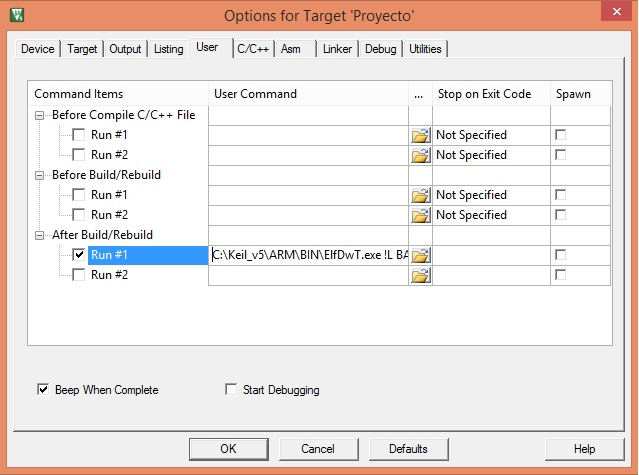
\includegraphics[width=100mm]{opctarget}
	\caption{Ventana de opciones para el proyecto }
	\label{cap1:005}
\end{figure}

Como última configuración, se da click nuevamente en \textbf{Barra de Herramientas} , \textbf{Project} y \textbf{Options for Target}. En la pestaña \textbf{Debug}, se da click en el botón \textbf{Settings} que se encuentra en la parte superior derecha de la ventana. En la pestaña \textbf{Flash Download} de la nueva ventana, en la sección de\textbf{ Download Function} se activa la casilla llamada \textbf{Reset and Run}. Este paso se muestra en la figura \ref{cap1:006}. Al finalizar se da click en \textbf{OK} de ambas ventanas. 

\begin{figure}[H]
	\centering
	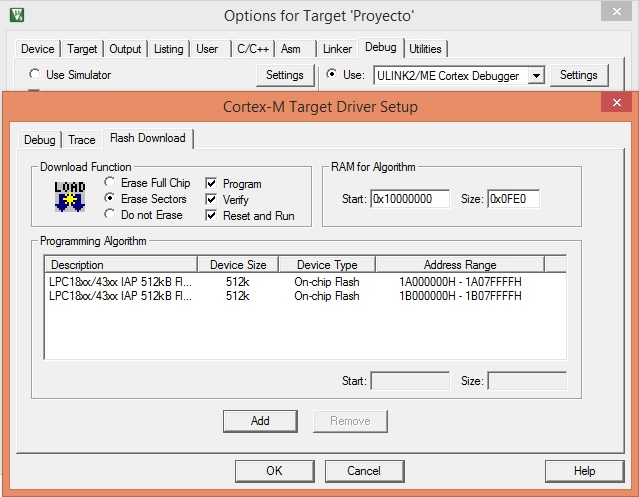
\includegraphics[width=100mm]{load}
	\caption{Ventana de opciones para cargar el proyecto }
	\label{cap1:006}
\end{figure}

Ya teniendo todas las configuraciones, se puede proseguir a dar click en la \textbf{Barra de herramientas} , \textbf{Project} , \textbf{ Rebuild All Target Files} . Se puede observar que todos los archivos: \textbf{main.c} , \textbf{LED\_MCB4300.c} , \textbf{RTX\_Conf\_CM.c} , \textbf{GPIO\_LPC43xx.c} , \textbf{SCU\_LPC43xx.c} y \textbf{system\_LPC43xx.c} tienen enlazados todas las librerías necesarias para cada uno. El último paso es dar click en \textbf{Barra de herramientas} , \textbf{Flash} , \textbf{ Download}. Con esto ya se pueden crear proyectos más elaborados teniendo en cuenta estos sencillos pasos. 

\chapter{Usando el Archivo de Encabezado para Plantilla: cmsis\_os.h}

El archivo cmsis\_os.h es un encabezado de plantilla que permite trabajar con todos los atributos de un Sistema Operativo en Tiempo Real, en este caso: el CMSIS-RTOS. Dicho archivo contiene la siguiente información  \cite{Keil}: 
\begin{itemize}
	\item Listas de comandos y acciones para definir hilos y otros objetos del núcleo del sistema operativo
	\item Definiciones de todas las funciones de la Interfaz de Programación de Aplicaciones (API)  de CMSIS-RTOS
	\item Definiciones de estructuras para parámetros y tipos de retorno de información
	\item Valores de estado y proridades usados por las funciones de la API de CMSIS-RTOS
\end{itemize}

\section{Funciones de CMSIS-RTOS}

El Sistema Operativo en Tiempo Real de CMSIS maneja funciones que pueden ser llamados desde hilos y desde Rutinas de Servicio de Interrupciones (ISR en inglés). Estas funciones se muestran a continuación \cite{Keil}:

\begin{itemize}
	\item Manejo de hilos
	\item Activación de señales
	\item Manejo de rutinas mutuamente excluyentes
	\item Manejo de semáforos
	\item Manejo de almacenes de memoria 
	\item Servicio de mensajes entre hilos
	\item Servicio de correos entre hilos
\end{itemize} 

\section{Convenciones de prefijos y manejo de hilos}

Es importante mencionar que las definiciones que tengan el prefijo \textbf{os} se refieren a aquellas que tienen asignado un único espacio para las funciones del CMSIS-RTOS. Y aquellas que tengan asignado el prefijo \textbf{os\_} no son usados por la API pero sí están referenciadas al archivo cmsis\_rtos.h 

La función de \textbf{Manejo de hilos} nos permite definir, crear y controlar las tareas de los hilos dentro del Sistema Operativo en Tiempo Real. La función \textbf{main} es una función de hilo especial que empieza al inicializar el sistema y tiene una prioridad inicial de \textit{osPriorityNormal}


Cada hilo puede estar en uno de los cuatro siguientes estados:

\begin{itemize}
	\item \textbf{ACTIVO:} Sólo un hilo a la vez puede estar en este estado
	\item \textbf{LISTO:} Aquél hilo que está a punto de pasar a ACTIVO está en este estado. Cuando un hilo está INACTIVO o EN ESPERA, aquél que esté en LISTO con la prioridad más alta pasa a estar ACTIVO.
	\item \textbf{EN ESPERA:} Aquél hilo que se encuentra esperando que un evento ocurra está en este estado.
	\item \textbf{INACTIVO:} Aquél hilo no creado o terminado está en este estado y no consumen recursos del sistema.
\end{itemize} 

En la figura \ref{cap2:001} se muestran los estados de los hilos, así como la transición entre estados.

\begin{figure}[H]
	\centering
	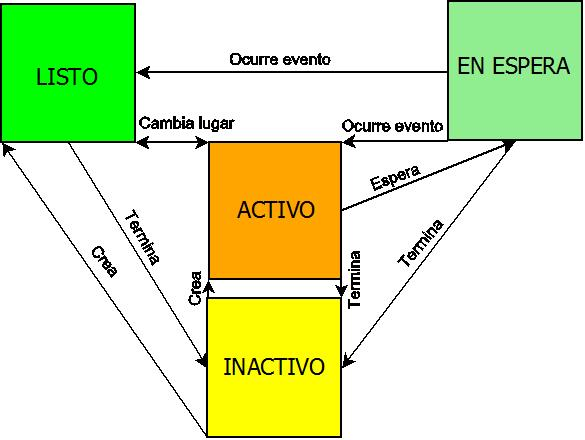
\includegraphics[width=100mm]{estados}
	\caption{Estados y transiciones de hilos}
	\label{cap2:001}
\end{figure}

Las funciones para poder utilizar los hilos de forma correcta están incluidos en la  tabla \ref{tabla2:001}.

\begin{table}[H]
	\begin{tabularx}{15cm}{|X|X|X|}
		\hline
		%\rowcolor[cmyk]{0,0,1,0}Abraham & Lapuerta\\
		\rowcolor[gray]{0.8}Función & Descripción & Ejemplo\\
		\hline
		%\rowcolor[rgb]{0,1,0}Roque & Fort\\
		\rowcolor[gray]{1}osThreadId & Define el nombre del hilo & osThreadId thread\_faseA;\\
		\hline
		\rowcolor[gray]{0.8}osThreadDef & Define atributos del hilo: nombre, prioridad inicial, número de instancias y
		tamaño para almacenar información & osThreadDef(faseA, osPriorityNormal, 1, 0); \\
		\hline
		\rowcolor[gray]{1}osThreadCreate & Empieza el hilo y lo coloca en estado LISTO, además define su argumento inicial. Sí este hilo tiene mayor prioridad que el hilo actual ACTIVO, este pasa a ocupar su lugar & thread\_faseA = osThreadCreate(osThread(faseA), NULL);\\
		\hline
		\rowcolor[gray]{0.8}osThreadTerminate & Termina la tarea del hilo y lo remueve & osThreadTerminate (thread\_faseA)\\
		\hline
		\rowcolor[gray]{1}osThreadGetId & Obtiene el nombre del hilo ACTIVO & id = osThreadGetId ();\\
		\hline
		\rowcolor[gray]{0.8}osThreadSetPriority & Cambia la prioridad del hilo & osThreadSetPriority (id, osPriorityBelowNormal);\\
		\hline
		\rowcolor[gray]{1}osThreadGetPriority & Obtiene prioridad del hilo & priority = osThreadGetPriority (id) \\
		\hline
		\rowcolor[gray]{0.8}osThreadYield & Pasa el control al siguiente hilo que está en estado LISTO & osThreadYield(); \\
		\hline
	\end{tabularx}
	\caption{Funciones básicas de hilos}
	\label{tabla2:001}
\end{table}

\section{Cambio de varias tareas por Algoritmo de Round-Robin}

El algoritmo de Round-Robin se usa en sistemas interactivos de tiempo compartido, en donde cada tarea puede realizarse en un tiempo máximo definido, llamdo \textit{cuantum}. Sí la tarea termina antes del tiempo máximo, deja el procesador por sí mismo. En caso contrario, sí ocupa todo el tiempo, el procesador expulsa el proceso.  \cite{Cobo}: 

La ventaja de ocupar el algoritmo de Round-Robin es que permite que se ejecuten varios hilos de forma casi-paralela. Esto es debido a que el cuantum que se define generalmente es de unos cuantos milisegundos y aparenta que las tareas se ejecuten de forma simultanea aunque realmente sea debido a que el RTOS asigna pequeños pedazos de tiempo a cada hilo.

Cuando termina el tiempo de ejecución del hilo o cuando éste termina su tarea, el CMSIS-RTOS cambia al siguiente hilo que está en estado listo y tiene la misma prioridad que la que terminó.Sí no hay hilos listos con la misma prioridad, se reanuda la ejecución del mismo hilo.

El cuantum se puede modificar dentro de las configuraciones del código llamado \textbf{RTX\_Conf\_CM.c} que se generan al compilar correctamente el proyecto. Se encuentran en la lista \textbf{System Configuration -> Round-Robin Thread switching [ACTIVAR] -> Round-Robin Timeout [ticks]}. Esto se muestra en la figura \ref{cap2:002}

\begin{figure}[H]
	\centering
	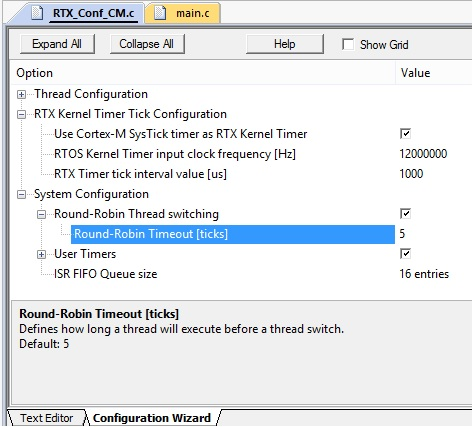
\includegraphics[width=100mm]{confround}
	\caption{Configuraciones para el algoritmo de Round-Robin}
	\label{cap2:002}
\end{figure}

En la figura \ref{cap2:003} se observa un diagrama de un sistema mínimo usando el algoritmo de Round-Robin.

\begin{figure}[H]
	\centering
	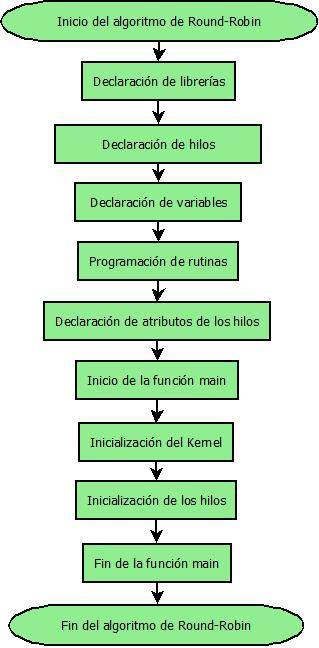
\includegraphics[width=60mm]{diaround}
	\caption{Diagrama de sistema mínimo usando algoritmo de Round-Robin}
	\label{cap2:003}
\end{figure}

\textbf{NOTA:}
El algoritmo de Round-Robin no se recomienda sí se quiere hacer programación con una estructura secuencial, debido al dificil control de ordenamiento de tareas. Se tiene el mismo problema sí dos o más hilos quieren acceder al mismo hardware: un hilo pondrá en espera al otro por lo que existirá un desfase de tiempos. Para estos casos, se recomienda utilizar otros algoritmos usando funciones de tipo mutuamente excluyentes o manejo de semáforos que se describen más adelante.

\section{Manejo de señales}

El manejo de señales permite controlar y esperar banderas de señales. Las funciones para poder utilizar estas señales de forma correcta están incluidos en la  tabla \ref{tabla2:002}.

\begin{table}[H]
	\begin{tabularx}{15cm}{|X|X|X|}
		\hline
		%\rowcolor[cmyk]{0,0,1,0}Abraham & Lapuerta\\
		\rowcolor[gray]{0.8}Función & Descripción & Ejemplo\\
		\hline
		%\rowcolor[rgb]{0,1,0}Roque & Fort\\
		\rowcolor[gray]{1}osFeature\_Signals  & Especifica el número de banderas máximas por hilo. Máximo pueden haber 31 banderas por hilo & 
		\#define osFeature\_Signals   8\\
		\hline
		\rowcolor[gray]{0.8}osSignalSet & Asigna una bandera a un hilo. Esta función se puede usar desde rutinas de interrupción & osSignalSet (hilo1, 0x0100); \\
		\hline
		\rowcolor[gray]{1}osSignalWait & Suspende la ejecución del hilo ACTIVO hasta que todas las banderas están activadas. Después regresa o coloca al hilo EN ESPERA. Las banderas usadas como eventos se limpian automáticamente. En esta función se puede especificar cuánto tiempo el sistema espera a la bandera. Pueden ser en milisegundos o usando \textbf{osWaitForever} para que espere hasta que la señal se active & osSignalWait(0x0100, osWaitForever); \\
		\hline
		\rowcolor[gray]{0.8}osSignalClear & Limpia las banderas especificadas de un hilo activo &  osSignalClear (hilo1, 0x0100);\\
		\hline
	\end{tabularx}
	\caption{Funciones del manejo de señales}
	\label{tabla2:002}
\end{table}

En la figura \ref{cap2:004} se observa un diagrama de un sistema mínimo usando las funciones del manejo de señales

\begin{figure}[H]
	\centering
	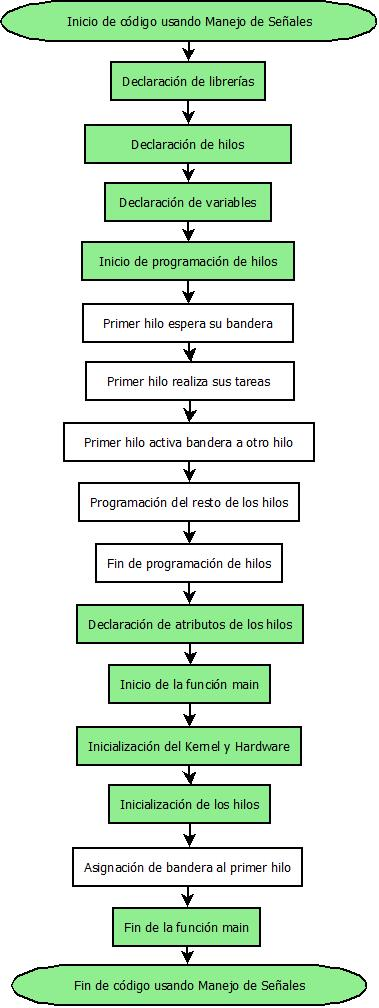
\includegraphics[width=60mm]{senales}
	\caption{Diagrama de sistema mínimo usando manejo de señales}
	\label{cap2:004}
\end{figure}

\textbf{NOTA:}
El manejo de señales resulta útil cuando se quiere hacer programación secuencial y se requiere que un hilo se enlace directamente a otro al terminar. En la práctica, esto resulta complejo sí se tienen muchos hilos y hay que enlazar un hilo con diferentes hilos dependiendo de las situaciones que se presenten. A continuación se describren otras funciones para esto.

\section{Manejo de rutinas mutuamente excluyentes}

El manejo de rutinas mutuamente excluyentes es usado para sincronizar la ejecución de hilos. Sobre todo se utiliza para proteger el acceso a un recurso compartido, por ejemplo: leds, memoria y demás periféricos.  En la figura \ref{cap2:005} se muestra el diagrama de estas funciones.

\begin{figure}[H]
	\centering
	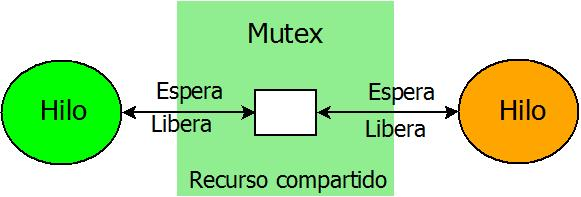
\includegraphics[width=60mm]{mutex}
	\caption{Rutinas mutuamente excluyentes usando la API de CMSIS-RTOS}
	\label{cap2:005}
\end{figure}

Las funciones para poder utilizar el manejo de rutinas mutuamente excluyentes de forma correcta están incluidos en la  tabla \ref{tabla2:003}.

\begin{table}[H]
	\begin{tabularx}{15cm}{|X|X|X|}
		\hline
		%\rowcolor[cmyk]{0,0,1,0}Abraham & Lapuerta\\
		\rowcolor[gray]{0.8}Función & Descripción & Ejemplo\\
		\hline
		%\rowcolor[rgb]{0,1,0}Roque & Fort\\
		\rowcolor[gray]{1}osMutexDef  & Define un objeto mutuamente excluyente & osMutexDef (Mutex1)\\
		\hline
		\rowcolor[gray]{0.8}osMutexId & Asigna un nombre único al objeto mutuamente excluyente & osMutexId mutex\_id \\
		\hline
		\rowcolor[gray]{1}osMutexCreate & Crea e inicializa un objeto mutuamente excluyente & mutex\_id = osMutexCreate  (osMutex (Mutex1)); \\
		\hline
		\rowcolor[gray]{0.8}osMutexWait & Espera hasta que un objeto mutuamente excluyente está disponible. En esta función se puede especificar cuánto tiempo el sistema espera al mutex. Pueden ser en milisegundos o usando \textbf{osWaitForever} para que espere hasta que el mutex esté disponible &   osMutexWait    (mutex\_id, 0);\\
		\hline
		\rowcolor[gray]{1}osMutexRelease &  Libera un mutex que fue obtenido por la función \textbf{osMutexWait}. Todos los demás hilos que estén esperando al mismo mutex ahora estarán en estado LISTO  & osMutexRelease(mutex\_id); \\
		\hline
		\rowcolor[gray]{0.8}osMutexDelete & Borra un objeto mutex. La función libera el espacio en memoria que estaba ocupado por el objeto. Después de esta función, el nombre o identificador del mutex ya no se podrá ocupar hasta que se vuelva a crear el objeto usando la función \textbf{osMutexCreate} &  osMutexDelete(mutex\_id);\\
		\hline
	\end{tabularx}
	\caption{Funciones de rutinas mutuamente excluyentes}
	\label{tabla2:003}
\end{table}

En la figura \ref{cap2:006} se observa un diagrama de un sistema mínimo usando las funciones de rutinas mutuamente excluyentes.

\begin{figure}[H]
	\centering
	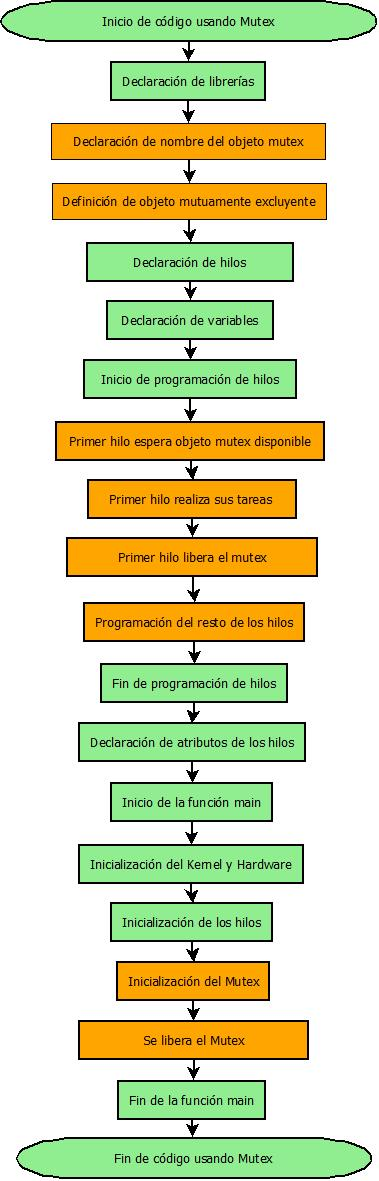
\includegraphics[width=60mm]{diamutex}
	\caption{Diagrama de sistema mínimo usando rutinas mutuamente excluyentes}
	\label{cap2:006}
\end{figure}

\textbf{NOTA:}
El manejo de rutinas mutuamente excluyentes es útil debido a que, a diferencia del manejo de señales, en estas se puede liberar el objeto mutuamente excluyente en una rutina y cualquier otra lo puede esperar, aún sin importar que sólo en algunas ocasiones esta se tiene que activar. Una de las desventajas de este método es que sí se quiere acceder a varios dispositivos en común, se vuelve complicado su manejo. Para ello se recomienda el manejo de semáforos que se describe a continuación. 

\appendix
\renewcommand{\appendixname}{Anexos}
\renewcommand{\appendixtocname}{Anexos}
\renewcommand{\appendixpagename}{Anexos}
\clearpage
\addappheadtotoc
\appendixpage
\chapter{Anexo I: Código para crear un nuevo proyecto}

\begin{lstlisting}[language=C]
#include "cmsis_os.h"
#include "LPC43xx.h"
#include "Board_LED.h"

/* Nombres de los hilos      */
osThreadId thread_faseA;                  
osThreadId thread_faseB;                 
osThreadId thread_reloj;                   

/* Primer hilo */
void faseA (void const *argument) {
for (;;) {
osSignalWait(0x0001, osWaitForever);
LED_SetOut	(0);
osSignalSet(thread_reloj, 0x0100);
osDelay(1000);
osSignalSet(thread_faseB, 0x0001);
//LED_Off(0);
}
}

/* Segundo hilo */
void faseB (void const *argument) {
for (;;) {
osSignalWait(0x0001, osWaitForever);
LED_SetOut	(254);
osSignalSet(thread_reloj, 0x0100);
osDelay(1000);
osSignalSet(thread_faseA, 0x0001);
//LED_Off(1);
}
}

/*Tercer hilo*/
void reloj (void  const *argument) {
for (;;) {
osSignalWait(0x0100, osWaitForever);  
LED_On(7);
osDelay(500);
LED_Off(7);
osDelay(500);
}
}

osThreadDef(faseA, osPriorityNormal, 1, 0);
osThreadDef(faseB, osPriorityNormal, 1, 0);
osThreadDef(reloj,  osPriorityNormal, 1, 0);

/* Funcion main */
int main (void) {

LED_Initialize();
thread_faseA = osThreadCreate(osThread(faseA), NULL);
thread_faseB = osThreadCreate(osThread(faseB), NULL);
thread_reloj  = osThreadCreate(osThread(reloj),  NULL);
osSignalSet(thread_faseA, 0x0001);
}

\end{lstlisting}

\begin{thebibliography}{X}
	\bibitem[Keil]{Keil} \textsc{ARM Ltd.}% y \textsc{H.D. Sherali},
	(2014, Septiembre 24)
	\textit{CMSIS-RTOS API: Generic RTOS Interface for Cortex-M processor-based devices}
	Recuperado de: http://www.keil.com
	
	\bibitem[Cobo]{Cobo} \textsc{Cobo, Pablo Martínex} %y \textsc{P. Wolfe},
	<<Sistemas operativos: teoría y práctica>>,
	\textit{Díaz de Santos}, %\textbf{8}, 
	págs. 64--65, 1997.
\end{thebibliography}

\end{document}